\section{什么是世界模型？}
\subsection{定义与主要性质}

\begin{figure}
\centering
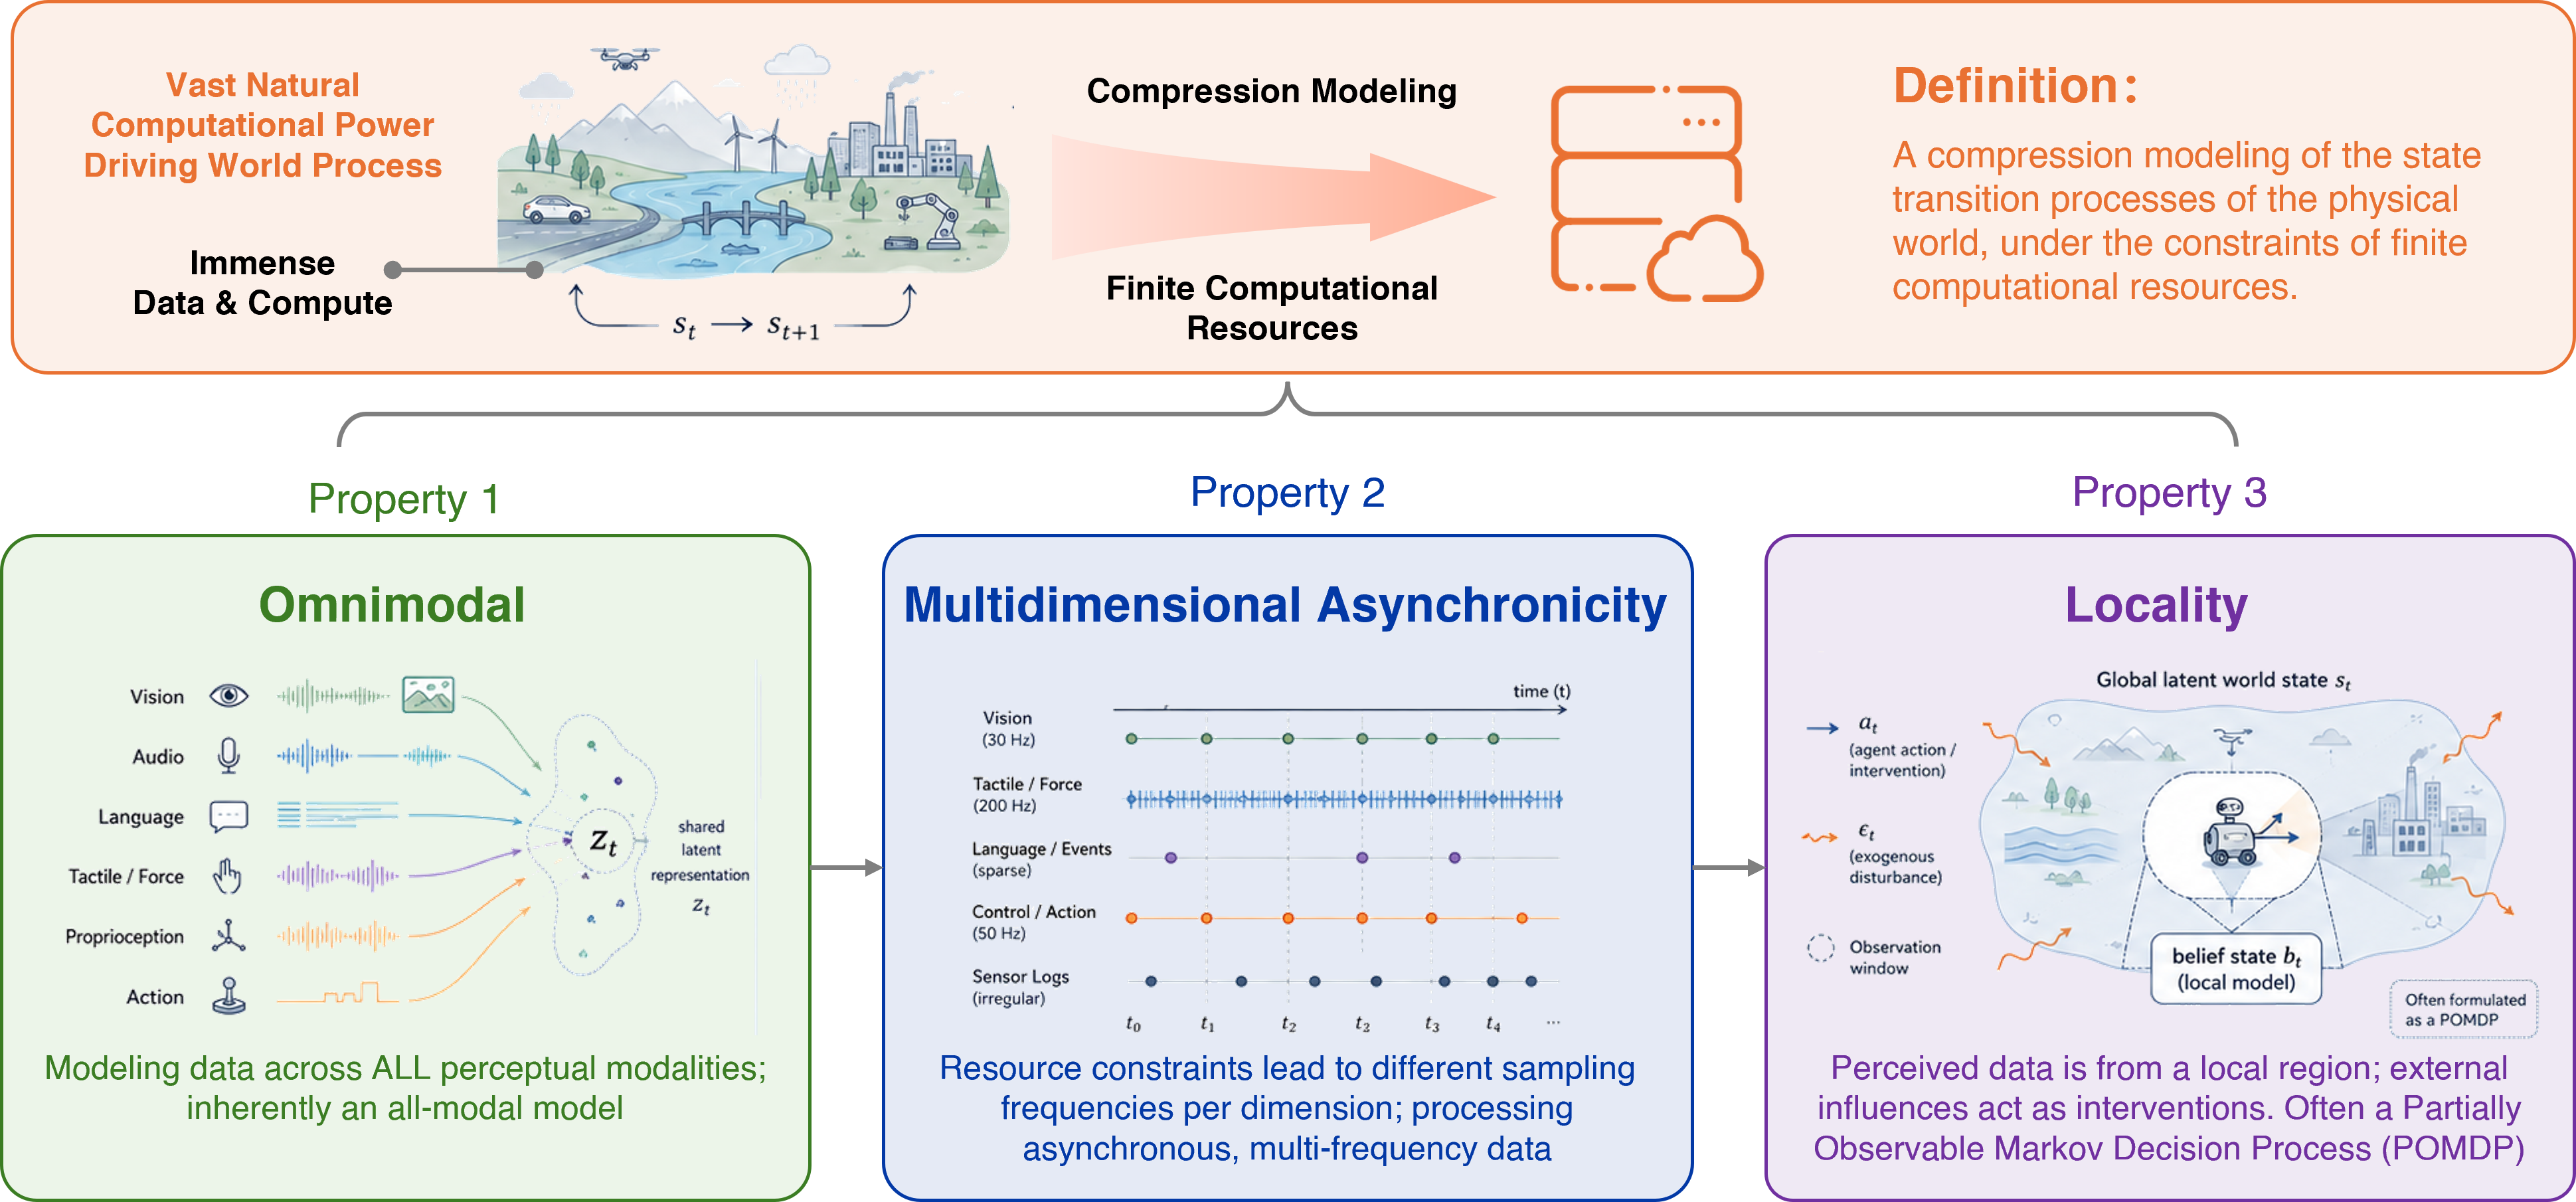
\includegraphics[width=\linewidth]{figs/WM-definition2.png}
\caption{世界模型的本质及其主要性质示意。}\label{fig:def-and-propoerties}
\end{figure}

本节专门从物理世界建模的角度，明确界定世界模型的概念，并概述其基本性质。

宇宙中一切物质与波的状态转移过程都客观存在，但驱动这些物理过程的自然计算能力极其庞大，难以估量。人类构建的系统无法复现这种无限复杂性，因此我们给出如下形式定义。

\begin{definition}[世界模型]
\label{def:worldmodel}
\textit{世界模型\footnote{依照这一定义，本文中的“世界模型”与“物理世界模型”（Physical World Model）含义相同，可以互换使用；但这并不意味着，在其他文献中，例如涉及交互式、三维几何一致的视频生成模型时，二者也具有相同含义。译注：原文此处写作“but this does mean”，与本句的转折关系及上下文不符，按“但这并不意味着”理解。}是在有限计算资源约束下，对物理世界状态转移过程进行的压缩建模。}
\end{definition}

如图\ref{fig:def-and-propoerties}所示，在这些内在计算约束下，通用物理世界模型具有三项主要性质：
\begin{itemize}
\item \textbf{全模态的作用范围（Omnimodal workscope）。}世界模型必须能够对所有感知模态的数据进行建模。它不限于文本或视觉，而在本质上是一种能够形成统一潜在表征的全模态基础模型。
\item \textbf{多维异步性（Multidimensional Asynchronicity）。}由于计算与感知资源有限，对物理世界各个维度的感知数据会以不同频率采样。因此，世界模型必须能够处理多维、异步（多频率）的序列数据。
\item \textbf{局部性（Locality）。}智能体的感知能力受资源限制，所采集的数据往往局限于某个局部区域。外部区域持续影响这一局部区域，构成干预。因此，从局部视角对世界建模，通常可表述为部分可观测马尔可夫决策过程（partially observable Markov decision process，POMDP）。
\end{itemize}

要理解这种局部、全模态近似的必要性，需要考察当前模型如何尝试回答关于现实的问题。当今人工智能领域占主导地位的世界模型，无论是潜在空间中的预测表征、用于游戏智能体的强化学习模型，还是用于具身模拟的视频预测模型，都遵循一种共同的生成式提问方式：给定当前观测，接下来会发生什么？真正的物理世界模型则重新界定了整个范式。基本问题从“将会发生什么”转向“正在发生什么、为什么会发生，以及将会发生什么”。这要求模型通过认识性推理（epistemic reasoning）\footnote{认识性推理是评估知识、信念及有理由支持的确信状态的逻辑过程，而非只关注世界的物理状态。它分析智能体如何依据部分观测、支持信息，以及关于其他智能体知道什么的元知识，构建、更新和评估内部表征。}理解物理系统的运行结构：发现系统自身的运行本体，识别离散的运行状态区间，确定正常与异常行为的边界，并刻画系统如何沿因果路径到达当前状态。

这一方法的意义，在于物理世界与数字世界有着巨大差异。数字数据一经产生，便可长期保持可读；多年前训练的语言模型，今天仍能回答量子力学问题。相反，物理系统内在地具有非平稳性，始终在变化。尤其是最重要的事件，如涉及安全的严重故障和罕见失效模式，可能从未出现在静态训练语料中。因此，静态世界模型不可避免地难以解决物理世界问题。我们需要一种架构，能够以通用基础表征为起点，自主、实时地适应各个应用中特有的物理规律。这样的动态系统应当具有\textbf{自洽性（self-consistency）}：当新的模态或数据通道进入时，世界模型仍能继续运行和演化，而不会面临崩溃。

归根结底，物理世界模型不仅是一台模拟引擎。它代表一种根本不同的智能形式：在局部观测与有限计算的约束下，深入理解物理世界、其持续演化及底层运行规律。

\subsection{智能体—环境循环}
\begin{figure}[t]
    \centering
    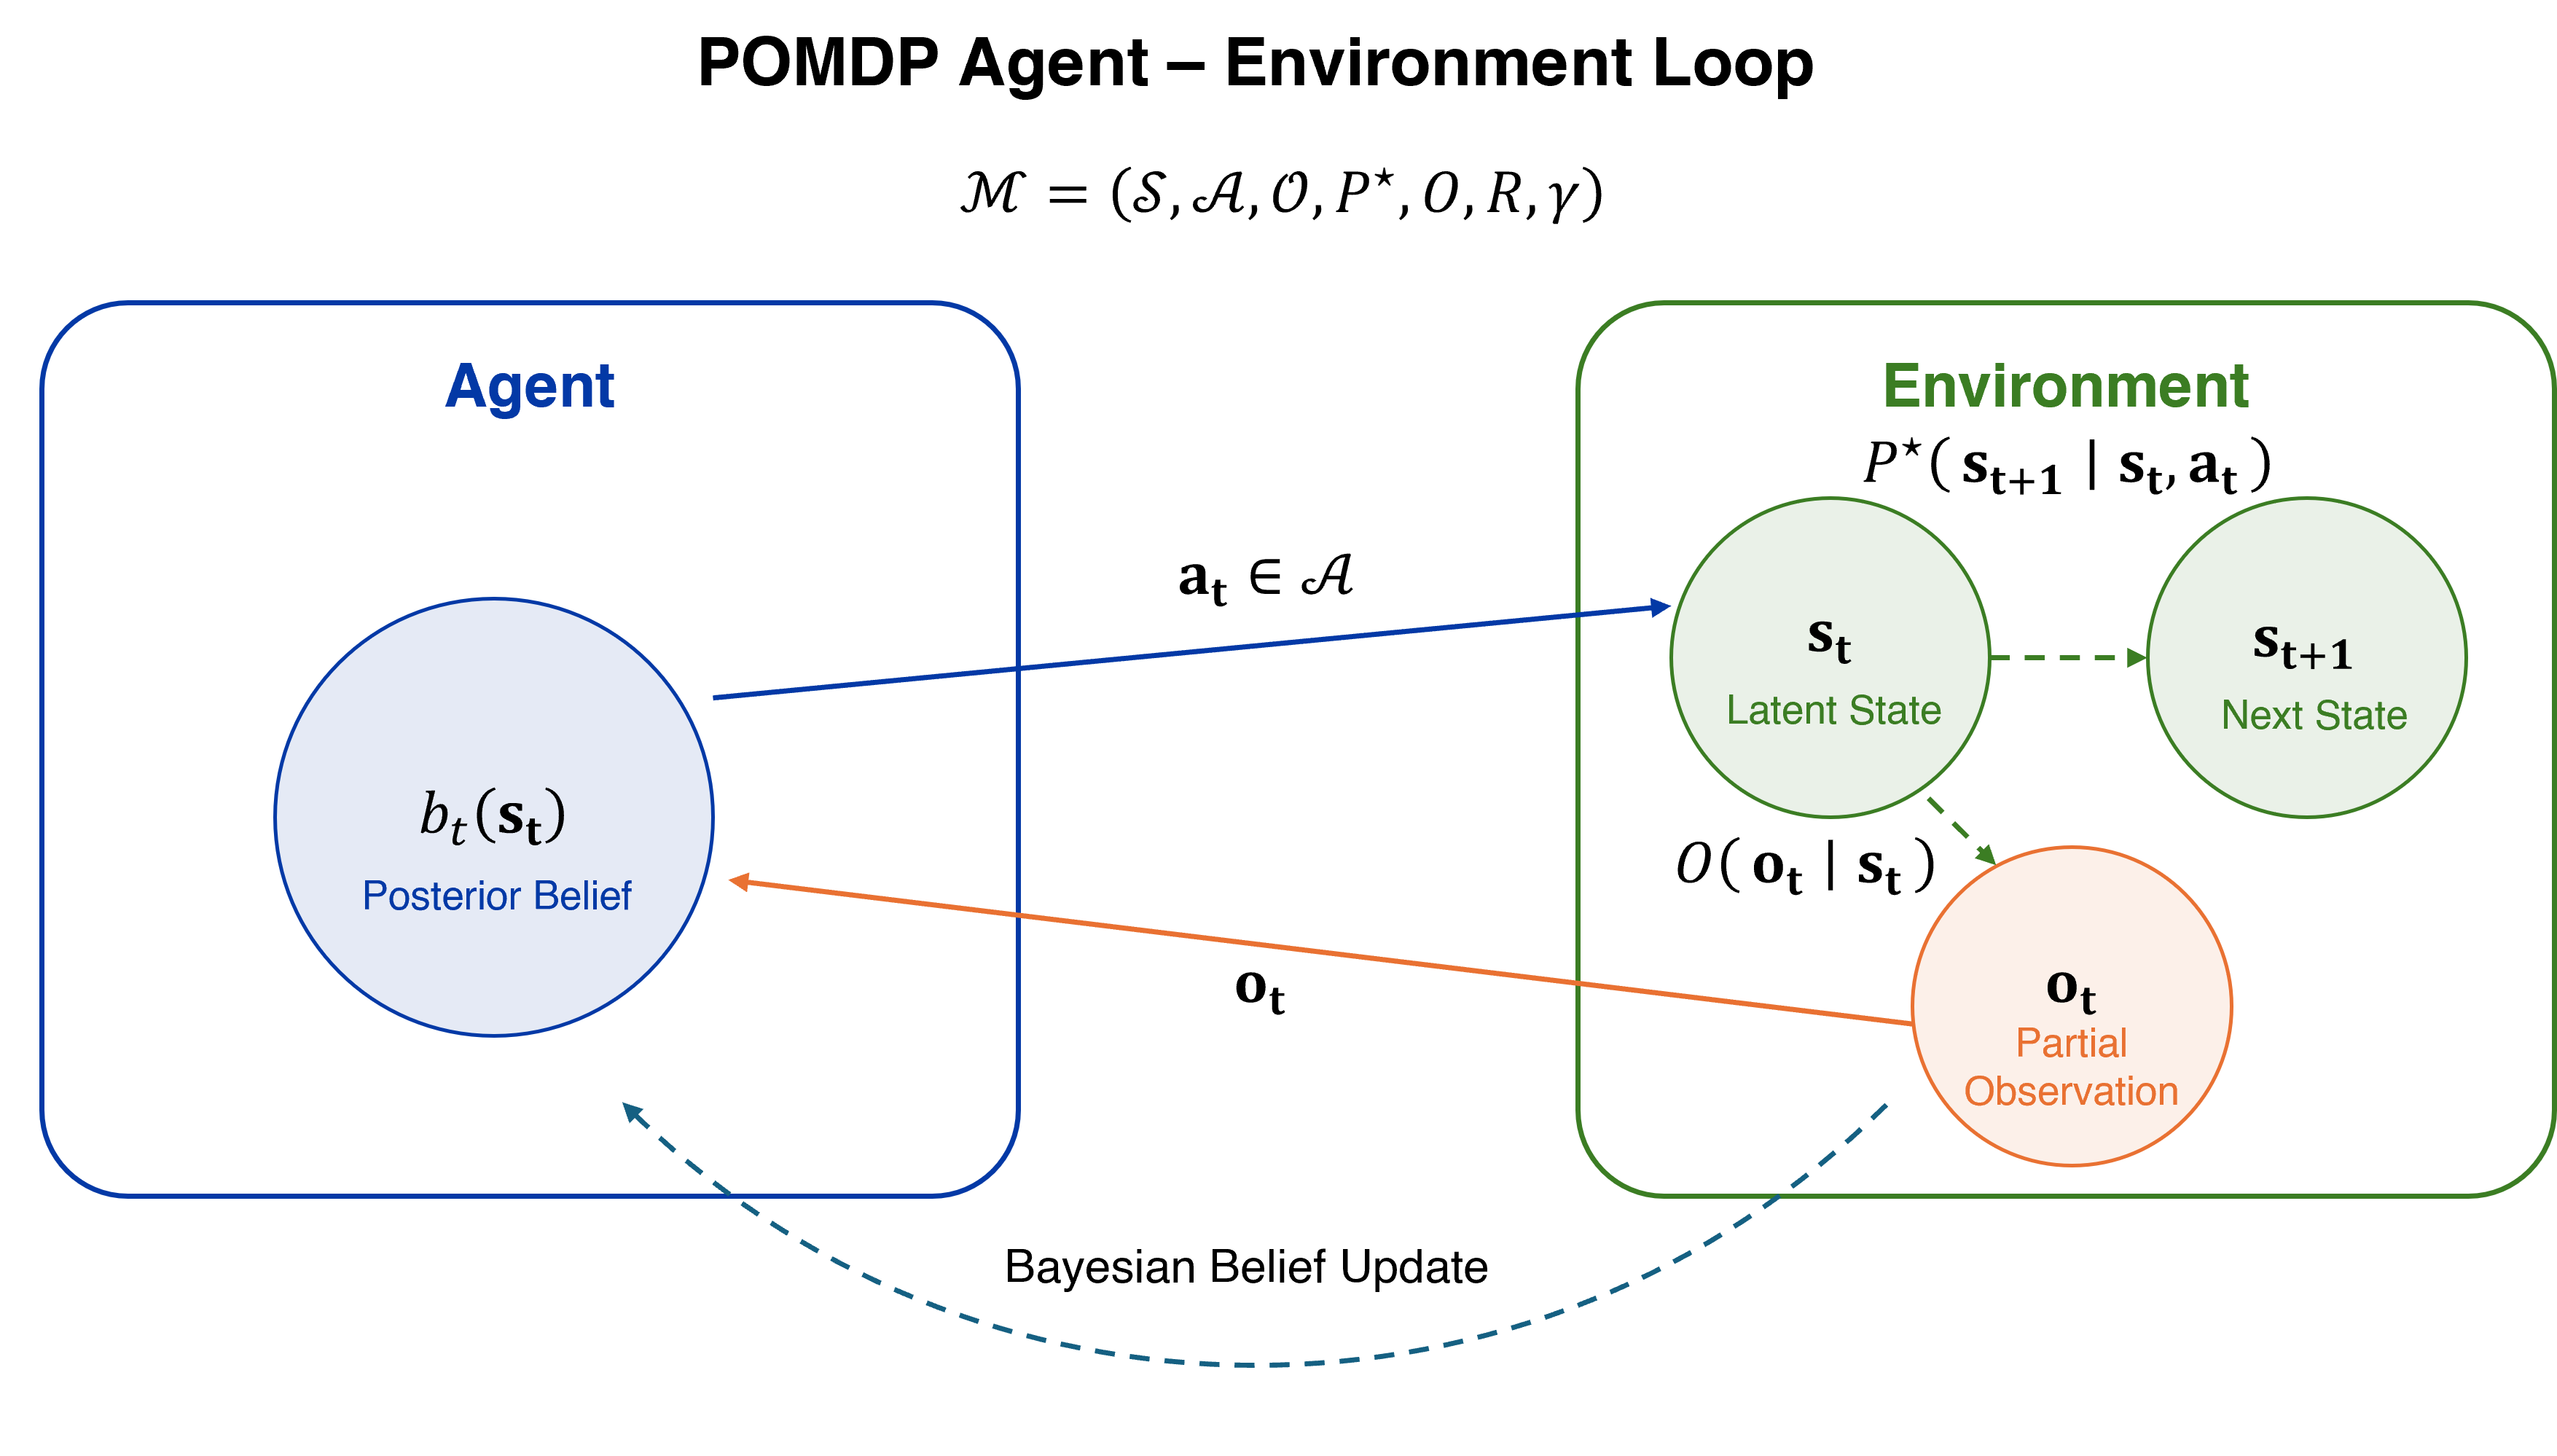
\includegraphics[width=0.8\linewidth]{figs/pomdp.png}
    \caption{采用本小节符号的POMDP智能体—环境循环示意。智能体维持后验信念$b_t(\mathbf{s}_t)$，选择行动$\mathbf{a}_t$；环境按照真实转移核$P^\star$演化，通过观测模型$O$产生部分观测$\mathbf{o}_t$；随后利用贝叶斯滤波更新信念。}
    \label{fig:pomdp-agent-environment-loop}
\end{figure}

一个在科学上有用的世界模型定义，应当从智能体与环境之间的序贯循环出发，而非从某个特定模型家族出发。自然的形式化方式是部分可观测马尔可夫决策过程（POMDP）$\mathcal{M}=(\mathcal{S},\mathcal{A},\mathcal{O}, P^\star,O,R,\gamma)$：环境处于潜在状态（latent state）$\mathbf{s}_t\in\mathcal{S}$，智能体选择行动$\mathbf{a}_t\in\mathcal{A}$，状态依照转移核（transition kernel）$P^\star(\mathbf{s}_{t+1}\mid \mathbf{s}_t,\mathbf{a}_t)$演化，智能体只能接收由观测模型$O(\mathbf{o}_t\mid \mathbf{s}_t)$生成的部分观测$\mathbf{o}_t\in\mathcal{O}$。真实状态通常是隐藏的，因此，有效行为不能只依赖原始观测，还需要对可能状态维持内部信念，并在新观测到来时更新信念。从这个意义上说，世界模型不只是像素、词元（token）或轨迹预测器，而是一个关于潜在状态、观测形成机制和行动条件动力学（action-conditioned dynamics）的内部模型，使智能体能够推断当前状况、想象接下来可能发生的事情，并在不确定性下评估干预。图\ref{fig:pomdp-agent-environment-loop}概括了这一循环及其核心变量。

这种表述也澄清了该术语的历史脉络。Craik早期的心智模型理论将智能理解为构建一种内部替代模型，在实际行动之前，先让它超前于现实运行\citep{craik1943nature}。Sutton的Dyna架构将这一思想转化为现代强化学习，把真实经验、模型学习、规划与行动显式地耦合在同一个循环中\citep{sutton1990dyna,sutton1991dyna}。近期的批评进一步强调：世界模型的目标不是穷尽式复现世界，也不只是生成视觉上可信的未来，而是为了有目的的推理和行动，模拟现实世界中可以采取行动的各种可能性\citep{xing2025critiques}。“可行动”这一限定至关重要。有用的世界模型不仅必须预测观测之间如何共同变化，还必须预测环境在干预下如何改变、哪些隐藏变量对控制重要，以及哪些不确定性仍未消除。在这一观点下，形式目标是学习一个对决策相关状态、转移与观测结构足够忠实的内部模拟器，使感知、反事实想象和策略选择都能在共同闭环中进行。

\subsection{理解与预测：世界模型的两种观点}
上述定义将物理情境下的世界模型界定为：在有限资源下对物理世界状态转移过程的近似，并强调全模态性、多维异步性和局部性三项主要性质。在这一定义之内，近期文献表明，“世界模型”一词有两种部分重叠、但哲学取向不同的含义\citep{ding2024understanding}。第一种观点主要将世界模型视为理解工具：它把感官数据压缩为持久的内部表征，揭示解释当前情境所需的实体、关系与机制。预测依然重要，但主要作为训练信号或一致性约束，促使表征捕捉正确的潜在结构。早期深度世界模型研究强调紧凑内部状态、记忆与潜在动力学，将其视为下游控制赖以建立的基础，体现的正是这一思想\citep{ha2018worldmodelsorig}。第二种观点主要将世界模型视为预测工具：根据模型向前推进世界、生成候选未来，以及为规划和决策提供前瞻的能力来评判它。LeCun的自主智能研究计划将这种预测式世界模型置于推理与行动的中心\citep{dawid2023autonomous}；Sora等大规模视频生成器则在可观测未来这一层面，使这种预测式理解尤为突出\citep{openai2024sora}。

这一区别会改变我们要求模型表征什么、优化什么、证明什么，因此十分重要。面向理解的模型通常偏好潜在抽象、以物体或关系为中心的结构、信念估计，以及对无关细节的不变性；其训练目标常强调表征学习、状态估计，或紧凑表征所具有的预测充分性；评估应检验所学状态能否为控制、解释和因果干预提供有用信息。面向预测的模型只要能够准确、可控地向前模拟，就可以容忍较弱的可解释性，因此常优先关注下一状态或下一观测的生成、长时域推演的持续可靠性、行动条件化，以及由外部标准判定的一致性。这两种观点也意味着不同的失效模式。模型可能推断出紧凑且与决策相关的状态，却生成视觉效果较差的渲染。相反，视频生成器可能生成极为逼真的未来，但如果不能保留隐藏状态、因果结构或干预含义，它仍无法成为控制所需的可靠模拟器\citep{xing2025critiques}。最强的系统最终将需要兼具二者：内部表征分离出恰当的潜在变量（latent variable），预测机制则将这些变量沿反事实未来向前推进。因此，这种分歧更适合被理解为：在特定架构中，哪种能力被视为首要能力，哪种被视为派生能力；而不是在两个不相容的定义之间做选择。

我们的观点是，对于物理世界模型，理解应当居于首位，预测应当服务于理解。无法识别潜在运行状态、因果结构以及与干预相关不确定性的模型，或许能够生成看似合理的未来，却仍不足以作为科学推理或具身控制的基础。另一方面，预测推演仍不可或缺，但其主要作用是通过反事实模拟检验并改进内部理解。从这个意义上说，最有用的世界模型并非单纯的未来生成器，而是把部分观测转化为可指导行动的理解，再利用预测支持决策的系统。

\subsection{功能分类：渲染器、模拟器与规划器}
区分面向理解和面向预测的世界模型，有助于澄清各自强调的能力，但尚未说明这些能力如何在行动系统中组织起来。因此，功能分类是有益的下一步：它根据世界模型在智能体—环境循环中的作用进行分解，而非按哲学侧重点划分。

李飞飞的功能分类可以重新表述为智能体—环境系统中三种互补的计算角色\citep{worldlabs2026taxonomy}。第一，渲染器是观测生成模型：以场景描述、交互历史或预期行动序列为条件，输出感知结果，最常见的是图像或视频。因此，它的功能是近似视觉上可信的观测分布，而非恢复环境完整的底层状态。第二，模拟器是承载动力学的模型，表征潜在或显式结构化的世界状态如何在干预下演化。它必须充分保留几何、物理约束、物体恒存性以及行动条件下的时间规律，才能支持可靠的前向预测。第三，规划器是决策模型，根据任务目标评估反事实未来并选择行动或行动序列。它不只是预测可能发生什么，还要决定应当追求哪一种可控未来。

这些角色自然地对应于POMDP闭环\citep{kaelbling1998planning}。真实环境状态不能直接获取，因此智能体对可能状态维持信念分布（belief distribution）。模拟器近似转移模型，在设想的行动下推进候选状态；渲染器近似观测模型，将这些状态投影为智能体随后可能接收的感官信息；规划器评估由此形成的、依赖信念的未来，以选择行动。选定行动执行后，环境产生新观测，修正智能体的信念并开启下一轮循环。因此，这三种功能既不是孤立模块，也不是相互排斥的模型类别。规划器查询模拟器，以比较行动后果，也可以调用渲染器，预期与任务相关的感知结果。反过来，规划器的干预决定环境的哪些方面变得可观测，从而产生可以改进感知预测与动力学估计的信息。它们的交互构成一个反复进行的推断、想象、干预与修正过程。

\begin{figure}
    \centering
    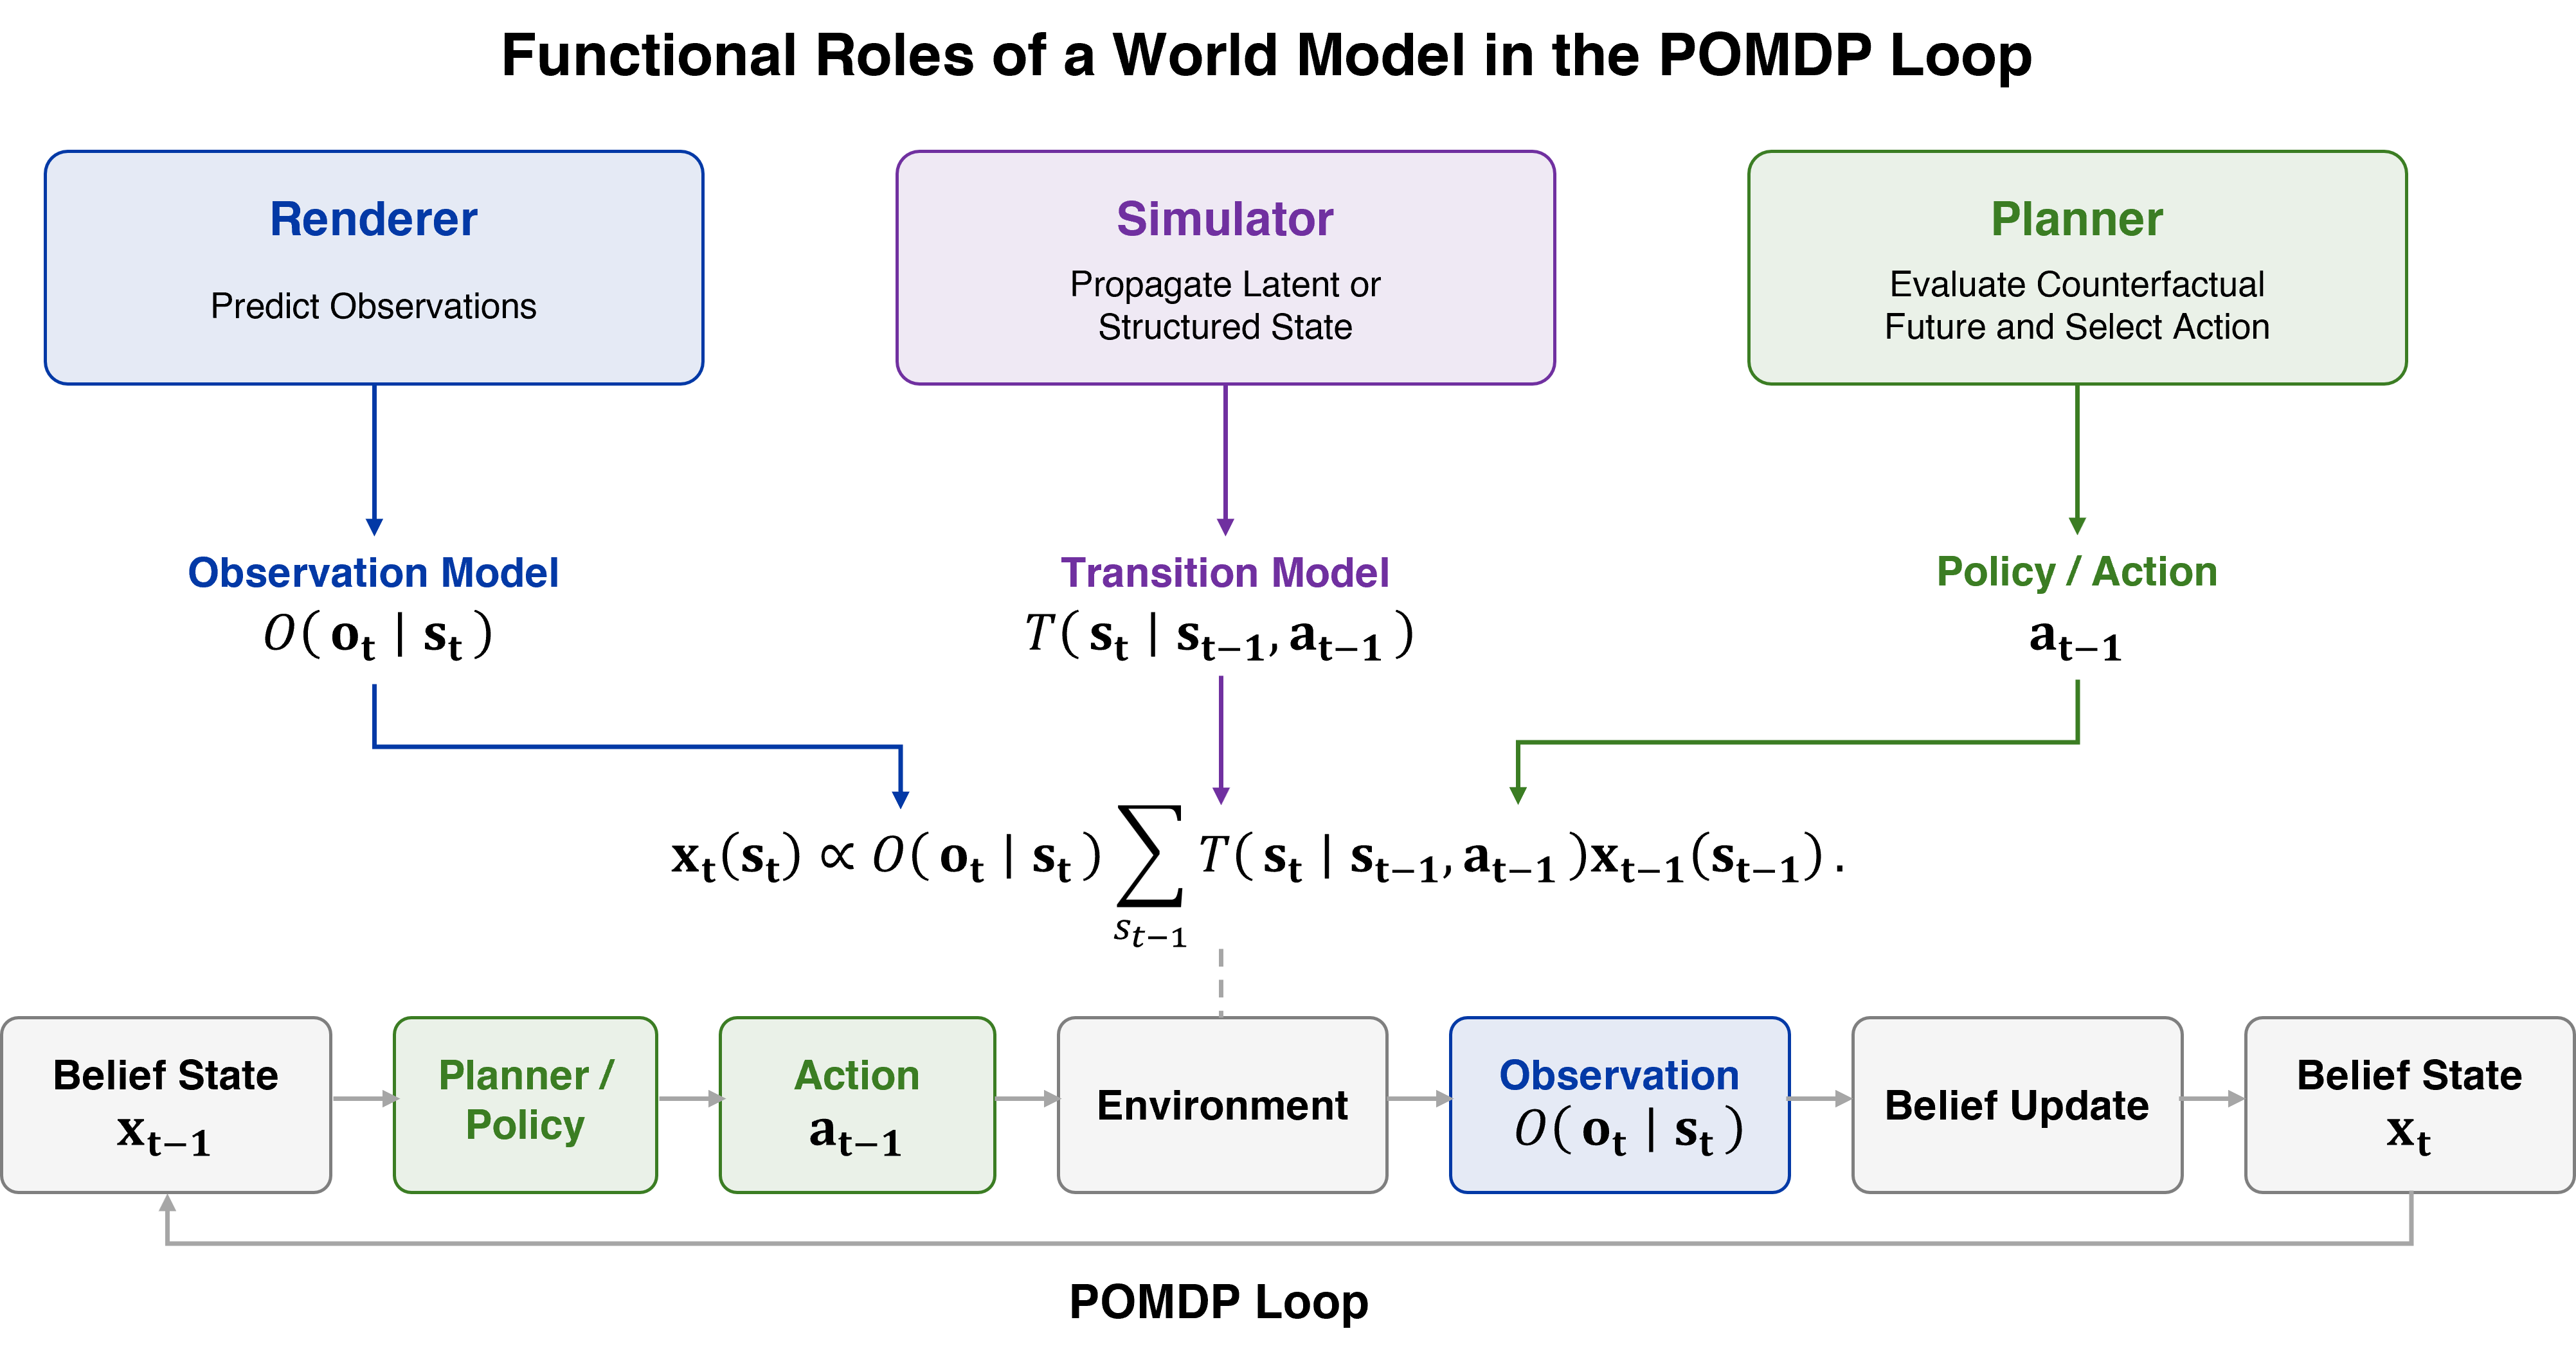
\includegraphics[width=0.96\linewidth]{figs/functional_roles3.png}
    \caption{世界模型在POMDP循环中的功能角色。}
    \label{fig:functional-roles}
\end{figure}

贝叶斯推断从规范角度解释了这一循环应当如何处理不确定性。在接收当前观测之前，智能体通过转移动力学传播上一时刻的后验，形成预测先验。随后，新观测按下式更新这一先验：
\begin{equation}
\mathbf{x}_t(\mathbf{s_t})\propto O(\mathbf{o}_t\mid\mathbf{s}_t)\sum_{s_{t-1}}T(\mathbf{s_t}\mid \mathbf{s_{t-1}},\mathbf{a_{t-1}})\mathbf{x}_{t-1}(\mathbf{s_{t-1}}).
\end{equation}
其中，$\mathbf{x}_t$表示后验信念，$T$是状态转移模型，$O$是观测似然。所得后验将积累的知识与当前信息结合起来，并显式保留不确定性，因此构成适当的决策信息基础。该后验随后又成为下一次预测先验的来源，使序贯贝叶斯滤波（Bayesian filtering）成为POMDP循环的推断支柱。理性规划应当在完整信念分布上优化期望效用，而非只考虑最可能的轨迹。因此，行动可以同时具有工具价值（instrumental value）和认识价值（epistemic value）：智能体可以为了实现外部目标而行动，也可以通过获取有信息量的观测来降低不确定性，或在两者之间权衡。先验编码跨环境学习得到、可重复利用的规律，后验使这些规律适应当前情境，反事实模拟则把二者与策略选择联系起来。因此，统一世界模型不应仅被理解为可能未来的生成器，而应被视为一个贝叶斯决策系统，持续地把不确定预测转化为依据观测信息、面向目标的行为。

\subsection{二维分类：功能与架构}
李飞飞的“渲染器—模拟器—规划器”分类与我们提出的分类处在不同的抽象层次。前者依据模型在智能体—环境循环中的功能角色分类：渲染器产生预测观测，模拟器在物理或动力学约束下推进世界状态，规划器依据目标选择行动。我们的框架则按模型的表征基础（representational substrate）与预测机制分类：观测层生成模型（observation-level generative model）直接在像素、视频等感知空间预测；潜在空间动力学模型（latent-space dynamics model）把观测编码为紧凑状态，并在表征空间中预测其演化；三维或其他结构化世界表征则显式建模几何、拓扑、物体、关系或物理属性。第一种分类问的是系统做什么，第二种问的是相关世界知识如何表示和计算。二者互补，而非相互竞争；一个模型通常应当在两个维度上各有一个或多个类别标签。

图\ref{fig:taxonomy}明确展示了这种多对多映射。Sora和Seedance位于观测层渲染器区域，因为它们对外提供的预测目标是视觉上可信的视频，而非结构显式、可独立查询的世界状态\citep{openai2024sora,gao2025seedance}。Genie 3的表征与输出仍位于观测层，但向三维世界表征方向延伸\citep{genie3}：它响应导航指令、智能体行动和可通过提示触发的世界事件，逐帧生成环境，从而支持交互式推演、反事实探索，以及智能体研究与训练。

JEPA家族位于潜在空间模拟器区域，因为其定义性预测目标是抽象的未来表征，而非重建像素\citep{assran2023ijepa,bardes2024vjepa}。VLA-JEPA将行动相关的潜在转移与连续行动生成耦合起来，从而把这一潜在预测机制扩展至规划器区域\citep{sun2026vlajepa}。Dreamer也位于潜在空间一列，但采用不同的生成式状态空间范式\citep{hafner2019dreamer}：从观测学习紧凑的行动条件动力学，并利用想象中的潜在轨迹训练演员（actor）与评论家（critic），以形成长时域行为。因此，在系统层面，它将潜在模拟器与通过想象训练的行动策略结合起来。更一般地，当行动条件潜在世界模型的预测与显式规划或控制目标耦合时，它们可以从模拟扩展至规划；用于以图像为目标的机器人规划的V-JEPA 2-AC，展示了这一点\citep{assran2025vjepa2}。

Marble主要位于三维／结构化表征区域\citep{worldlabs2025marble,kerbl20233dgaussians}。其高斯泼溅（Gaussian Splatting）表征支持高保真渲染与新视角合成（novel-view synthesis），碰撞网格则提供可供下游物理引擎使用、适于模拟的几何。因此，它连接了渲染与模拟，但不应将碰撞表征本身等同于完整的、学习得到的物理动力学模型。

Cosmos 3在图中表示为横跨多个区域的能力分布，而非分类中的单一位置\citep{nvidia2026cosmos3}。在共享的全模态架构中，其视听生成模式承担渲染器功能，行动条件前向动力学模式承担模拟器功能，策略模式则联合预测行动及其预期视觉后果。因此，图\ref{fig:taxonomy}中的位置反映了这样一个事实：不同的输入输出配置与后训练过程，可以从共享模型骨干中展现不同的功能角色。综合来看，对能力日益增强的世界模型，更合适的刻画方式是描述其运行配置与能力分布，而非将一个不可分割的模型名称归入单一类别。

出于同样原因，我们不把当前备受关注的世界行动模型（WAM）视为第四种实现类别。如图\ref{fig:taxonomy}中水平的WAM区域所示，WAM是用于具身决策、横跨多种架构的功能范式，而非与三列架构并列的表征基础。它的定义性特征是将预测式状态建模与行动生成耦合。在系统层面，WAM建模预期未来状态与行动之间的关系，即使这一关系通过级联分解实现，而非完全统一的网络。

WAM可以通过显式未来视频进行推理，如视觉规划流程；也可以通过紧凑的潜在未来表征或轨迹进行推理；还可以通过光流、三维点流、RGB-D轨迹等结构化空间表征进行推理。因此，它可以借助观测层、潜在空间或结构化世界模型实现。在李飞飞的功能维度上，WAM主要面向规划，但通常同时跨越规划器与模拟器功能，因为未来状态预测是行动生成的构成部分，而非仅仅起辅助作用。把WAM视为以预测式行动生成为中心的功能家族，可以避免混淆输出功能与实现基础，也允许对级联系统和联合系统进行有意义的比较：前者先预测未来状态表征，再导出行动；后者共同建模状态与行动轨迹。

\begin{figure}
    \centering
    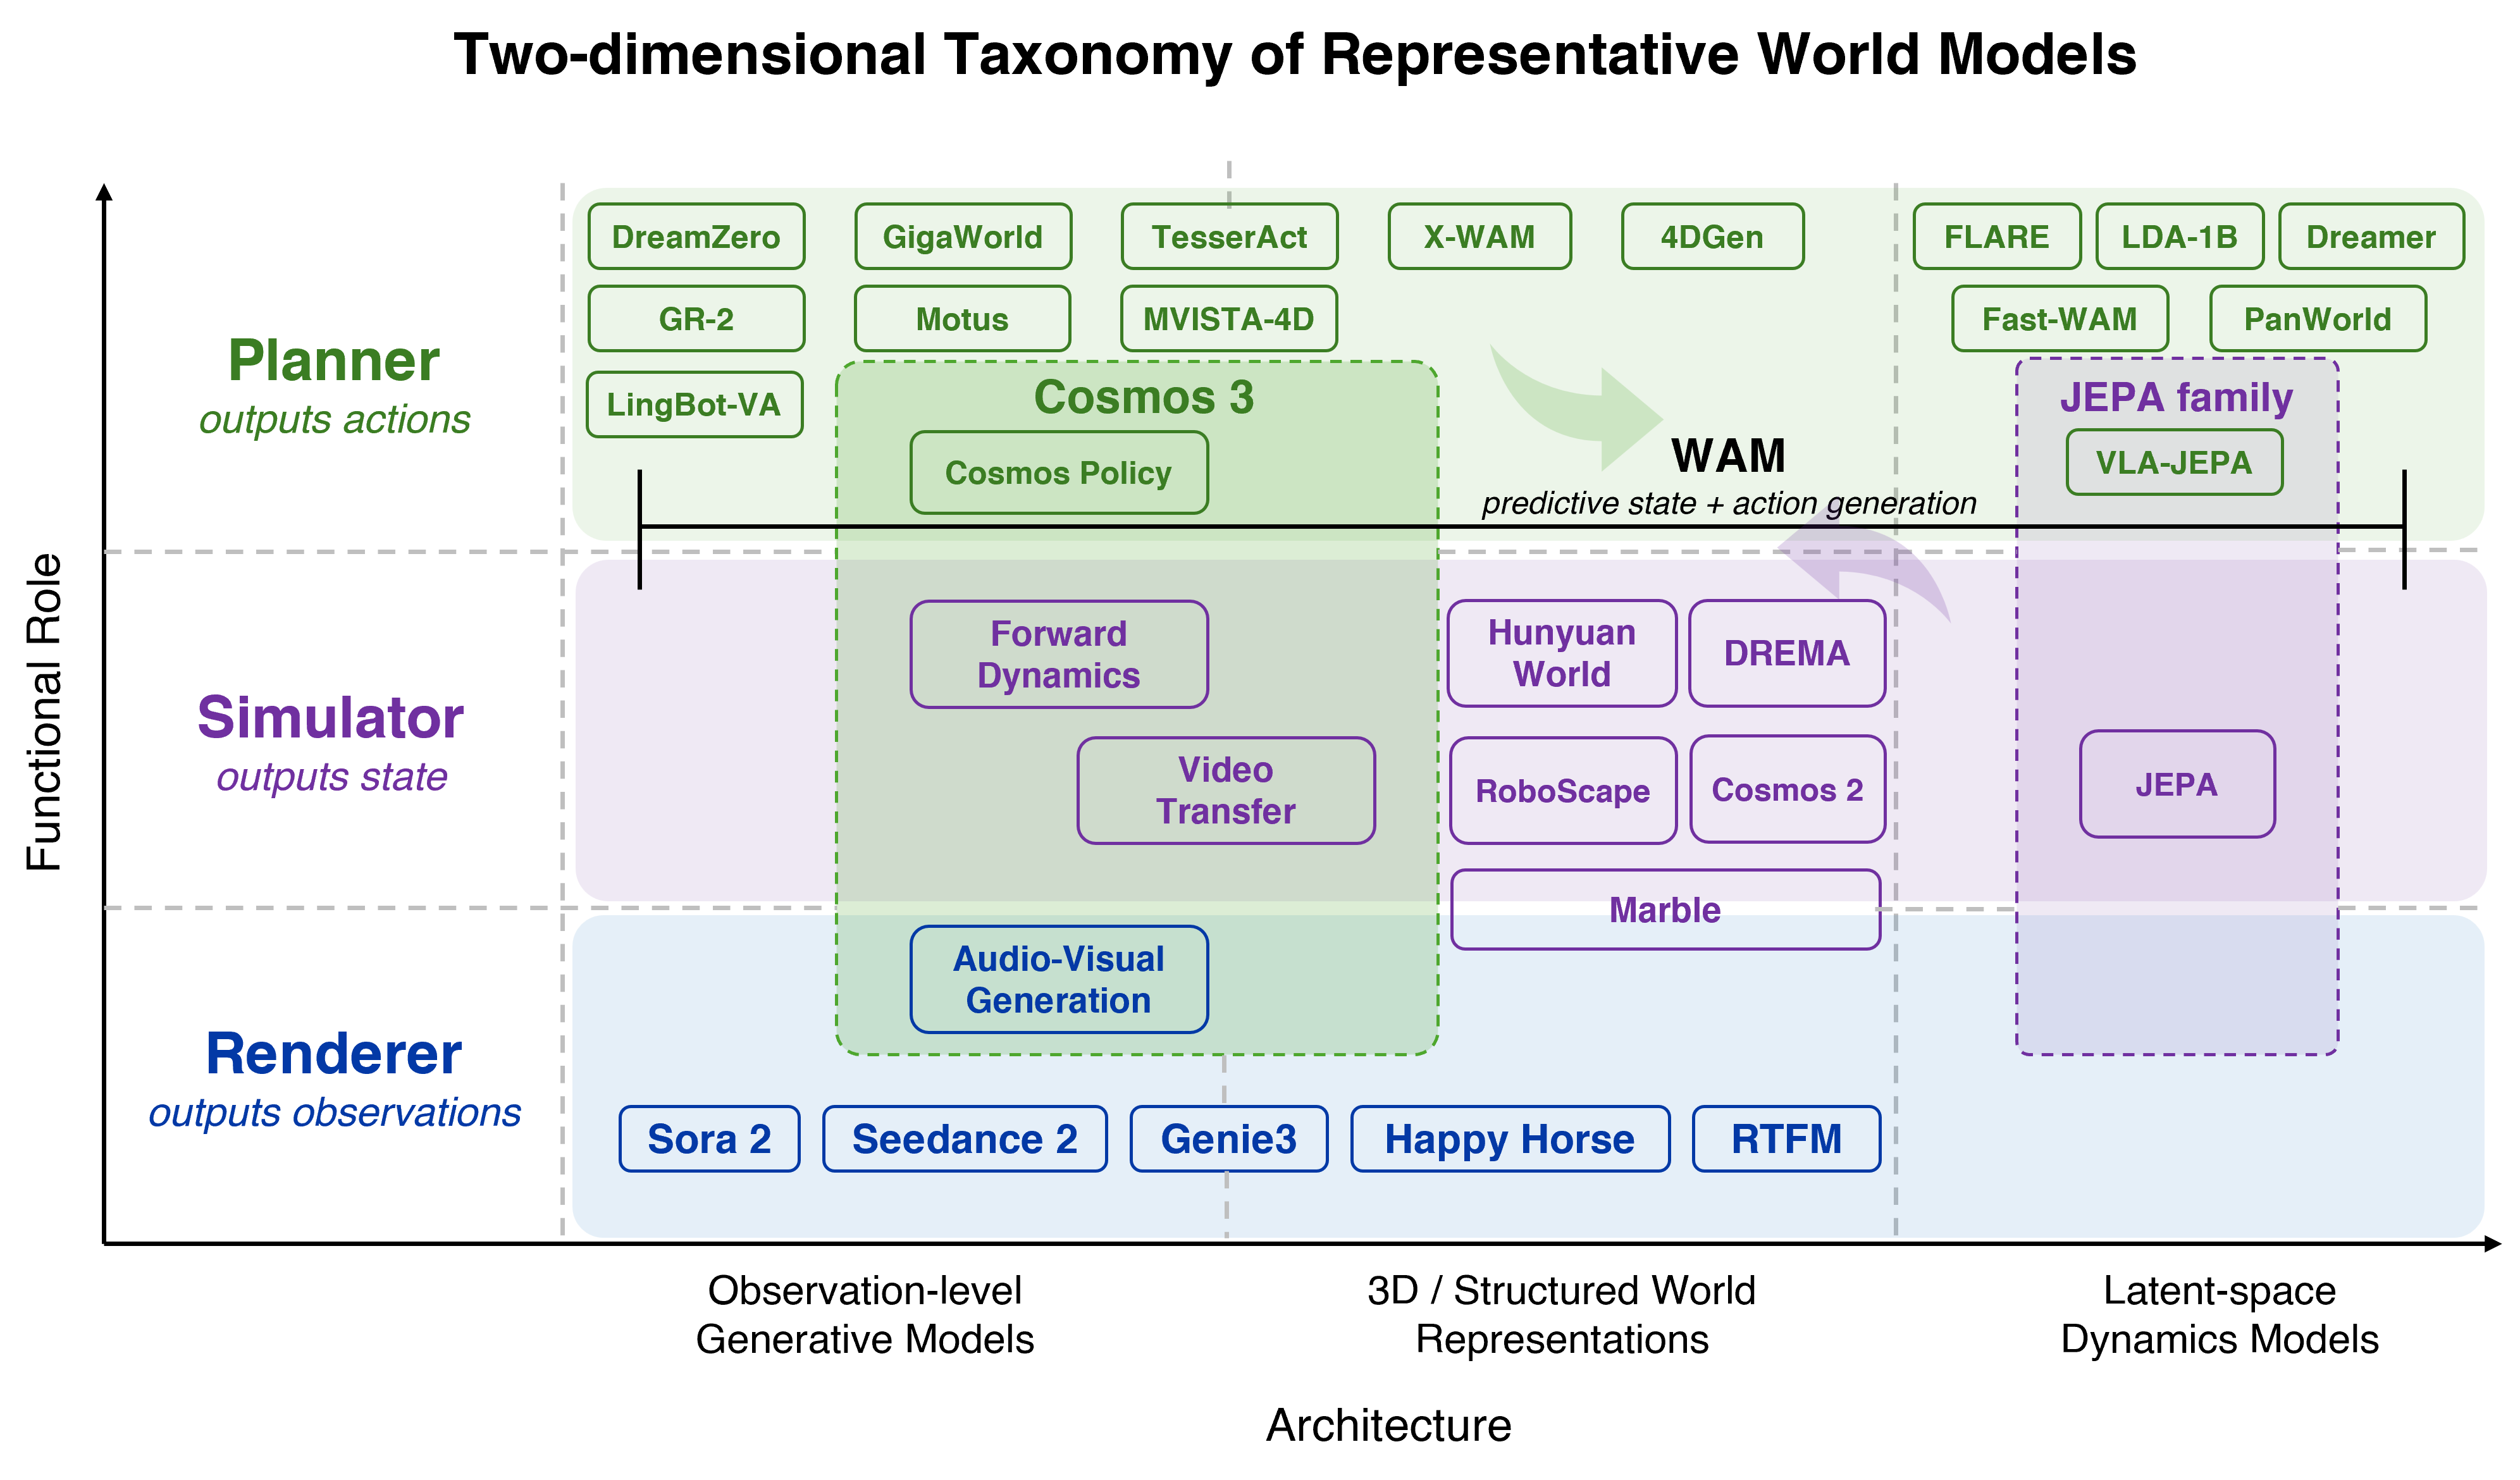
\includegraphics[width=0.96\linewidth]{figs/Taxonomy3.png}
    \caption{二维分类：功能与架构。}
    \label{fig:taxonomy}
\end{figure}

\subsection{将世界模型扩展到物理环境之外}
前述讨论主要仍局限于日常宏观环境，包括场景、机器人、车辆和可操作物体。更广泛的研究议程应当探讨：能否为科学领域构建类似的世界模型。在化学中，视任务而定，状态可以包括分子种类和结构、反应进程以及相关动力学或热力学变量；观测可以包括光谱、色谱或测得的产率；行动则可对应实验中可控的干预。在生物学中，相关状态可以通过层级或多尺度表征，跨越分子网络、细胞表型、组织及生物体层面的过程；干预可包括遗传扰动、给药及其他受控操作。在天文学中，潜在天体物理状态通过仪器被间接观测，而规划可能涉及根据天体物理动力学及仪器相关观测模型，选择观测目标、仪器与时间安排。

现有科学模型已经展示了这一表述的部分内容。在气象学中，GraphCast学习全球大气状态上的自回归转移模型，通过反复向前推进数百个大气变量，生成中期预报\citep{lam2023graphcast}。在本文分类中，它可被理解为结构化科学模拟器；但由于它不选择干预，也不闭合预测与行动之间的循环，因此不是智能体式世界模型。在分子尺度，MDGen学习分子动力学轨迹的生成模型，可以通过条件化用于前向模拟、转移路径生成及轨迹上采样\citep{jing2024mdgen}。它同样体现了学习式科学动力学建模，但本身不构成完整的实验规划系统。这些案例表明，即使没有明确使用“世界模型”这一名称，状态表征、时间推进、考虑不确定性的生成以及条件预测等世界建模组成部分，也已在各个科学领域涌现。在这些领域中，科学世界模型不能只生成看似合理的测量结果，还应捕捉机制性结构或其他具有科学意义的结构，在适用时遵守已知物理约束与不变量，量化不确定性，支持反事实干预，并在实际约束下帮助选择信息量大或效用最大的实验。完整的智能体式科学世界模型，还应把这些能力连接到实验循环：提出假说或干预，预测结果，执行实验，再依据新信息更新模型内部状态。

更广泛、也更具推测性的扩展，是有明确边界的社会系统\citep{zhou2025socialworldmodels}。我们将这一概念限制在参与者、交互规则、观测通道、干预空间和时间跨度都有清楚定义的系统，如小型团队、小型组织或界定狭窄的制度流程。这些系统可以建模为部分可观测的多智能体动力过程。候选潜在变量可以包括激励、信念、组织结构、资源约束和交互网络；观测可以包括通信、交易和绩效记录；干预可以包括任务分配、组织重构或协商达成的行动。在这些边界内，社会世界模型可以为团队协调与组织运营提供情景分析。

继续讨论之前，我们强调，本文的主要研究对象是物理世界的世界模型，而非社会系统。这里对社会领域的讨论，只是用来澄清适用范围和潜在局限的概念性扩展，不应被理解为本文的中心研究对象。

这种表述不应未经限定地扩展到国家、人口群体或全社会预测。大规模社会系统具有开放性、反身性和非平稳性，其规范性目标也存在争议：预测与干预可能改变被建模的行为，智能体可能对模型做出策略性反应，不同群体可能追求不相容的目标。此外，信念、偏好和意图等变量只能被部分观测，也可能依赖存在争议的理论假设。因此，当制度变化或公众知晓预测时，历史预测准确性并不能保证干预效果可靠。

其中的伦理与治理风险相当大。根据通信和行为记录推断潜在状态，可能助长侵犯隐私的监控；含有历史偏差的数据可能再现歧视或不平等的风险分配。模型输出用于分配机会、执行政策或塑造行为时，还可能产生施为性影响，形成自我强化的反馈循环\citep{perdomo2020performative}。因此，社会世界模型应显式表示不确定性，记录其因果与规范假设，并接受隐私保护、偏差审查、分布变化（distribution shift）测试和人工监督。它们应被视为有明确边界的决策支持工具，而非社会预言机；不应被用于不受约束的人口规模预测、大规模画像、自动化治理，或涉及个人和社会群体的高风险决策。

为避免术语泛化，“世界模型”这一名称应保留给以下系统：维持状态的内部表征，建模时间转移及适用时的干预条件转移，并生成可检验的预测。在这些限制下，二维框架仍可用于边界明确、具有操作性定义的社会领域。一个不受约束、试图建模整个国家或社会的模型，不应仅凭其规模或预测雄心，就被视为世界模型。
